\documentclass[11pt,a4paper]{article}

\usepackage[utf8]{inputenc}

\usepackage{natbib}

\usepackage[margin=1.1in]{geometry}
\setlength{\parskip}{0.5em}
\parindent 0pt

\usepackage{setspace}
\onehalfspacing

\usepackage{amsmath}
\usepackage{bm}

\usepackage{color}
\definecolor{darkblue}{rgb}{0,0,.5} 
\usepackage{hyperref}
\hypersetup{colorlinks=true, linkcolor=darkblue, citecolor=darkblue, filecolor=darkblue, urlcolor=darkblue}


\usepackage{multirow}
\usepackage{rotating}
\usepackage{booktabs}
\usepackage[labelfont={bf,small},textfont={small},justification=RaggedRight,margin=0pt]{caption}


\usepackage[framemethod=tikz]{mdframed}

\newmdenv[shadow=true,shadowcolor=black,font=\sffamily,rightmargin=8pt]{shadedbox}

\usepackage{tikz}
\usetikzlibrary{arrows,automata,shadows}

\usepackage{fancyhdr}

\renewcommand{\rmdefault}{ptm}
\pagestyle{fancy}

\lhead[]{\today}
\chead[]{}
\rhead[]{mmarbach@mail.uni-mannheim.de}
\rfoot[\thepage]{}


% History:
% - first version June, 2011
% - revisited after consolidating my notes on Gibbs Sampling, included statement on sampling 
% - included marg. data aug. statement in June 2013

\newcommand{\f}{\mathit{f}}
\newcommand{\LL}{\mathit{L}}


\begin{document}

\textbf{Bayesian Probit Model}\footnote{Notes by Moritz Marbach. Comments welcome.} \\

Let there be $I$ choices. For the purpose of the following discussion, it is useful to state the model from a latent variable perspective. Let $y_{i}^{*}$ be an unobserved random continuous variable which is drawn from a normal density with a mean parameterized by a linear predictor $\mathbf{x}_i \boldsymbol{\beta}$ and an variance term $\sigma$. $\mathbf{x}_i$ is a vector of length $K$ and $\boldsymbol{\beta}$ a vector of $K$ parameters. 

We only observe the latent variable in terms of a binary state: If $y_{i}^{*}$ is strictly smaller than 0, we observe $y_{i}=0$, for values larger than $\tau$, we observe $y_{i}=1$. The probability model of this can be written as:

\begin{equation}
\begin{split}
y^{*}_i &\sim \mathrm{\mathbf{N}}(\textbf{x}_i \boldsymbol{\beta} ,\sigma) \\
y_{i} &= \left \{
\begin{array}{ll}
	0 & \quad \text{if $y_{i}^{*} < 0$ }\\
	1 & \quad \text{otherwise}\\
\end{array} \right..
\end{split}	
\end{equation}

In order to identify the model $\sigma$ is usually set to one. To complete the Bayesian model, it is necessary to specify a prior distribution for the coefficients. It is usually assumed that they are from a multivariate normal distribution: 

\begin{equation}
\begin{split}
\boldsymbol{\beta} &\sim \mathrm{\mathbf{N}}(\textbf{b}_0, \textbf{B}_0) \\
\end{split}
\end{equation}

The posterior distribution can not be marginalized analytically. A Gibbs sampler was first suggested by \citet{Albert.Chib.1993} and can be motivated using data augmentation and the directed acyclic graph (DAG) of the model. 

A data augmented DAG representation of the model appears in figure \ref{fig:ProbitDAG}. Each node is a random variable. Rectangular nodes indicate observed variables, circle nodes represent unobserved variables. An arrow indicates the dependencies between these variables. The DAG helps to derive the full conditionals for the Gibbs sampler. \citet{Lauritzen.et.al.1990} have shown that the conditional densities of any node $(\theta_1, .... \theta_j,...\theta_J)$ in a DAG $\mathcal{G}$ can be written as:

\begin{equation}
\f(\theta_j | \theta_{\neg j}) \propto \f(\theta_j | \mathrm{parents}[\theta_j]) \times \prod_{w \in \mathrm{chidren}[\theta_j]} \f(w|\mathrm{parents}[w]),
\end{equation}

where $\theta_{\neg j}$ denotes all nodes in $\mathcal{G}$ other than $\theta_j$. 


\begin{figure}[!ht]
\centering

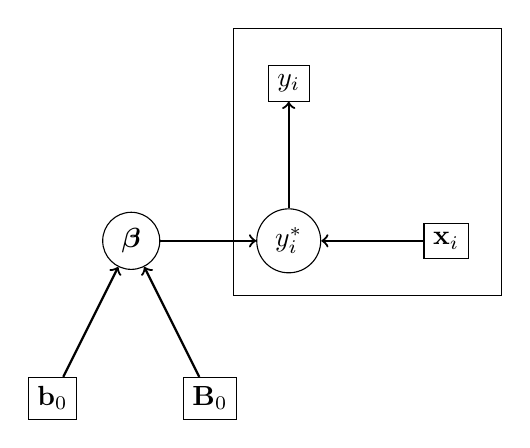
\begin{tikzpicture}[scale=2]
\tikzstyle{every node}=[draw,shape=circle];
\draw[fill=white] (0.65, -0.35) rectangle (2.35, 1.35);
\path (-0.5,-1) node[rectangle]  (b0) {$\mathbf{b}_0$};
\path (0.5,-1) node[rectangle]  (B0) {$\mathbf{B}_0$};
\path (0,0) node (beta) {$\boldsymbol{\beta}$};
\path (1,0) node (ystar) {$y_i^{*}$};
\path (2,0) node[rectangle]  (x) {$\mathbf{x}_i$};
\path (1,1) node[rectangle]  (y) {$y_i$};
\draw[thick,->] (beta) -- (ystar);
\draw[thick,->] (ystar) -- (y);
\draw[thick,<-] (ystar) -- (x);
\draw[thick,->] (b0) -- (beta);
\draw[thick,->] (B0) -- (beta);
\end{tikzpicture}

\caption{A directed acyclic graph representation of a probit model.} \label{fig:ProbitDAG}
\end{figure}

\newpage 

Given the DAG in figure \ref{fig:ProbitDAG}, we can derive the full conditional densities for the two unobserved variables: 

\begin{equation}
\begin{split}
\f(\boldsymbol{\beta} | \mathbf{b}_0, \mathbf{B}_0, \mathbf{y}^{*}, \mathbf{y}, \mathbf{X} ) &= 
	\f(\boldsymbol{\beta} | \mathbf{b}_0, \mathbf{B}_0) \times \prod_{i=1}^{n} \f(y_i^{*}|\mathbf{x}_i, \boldsymbol{\beta})\\
\f( y_i^{*} | \mathbf{b}_0, \mathbf{B}_0, \boldsymbol{\beta}, \mathbf{y}, \mathbf{X} ) &= 
	\f(y^{*}_i | \mathbf{x}_i, \boldsymbol{\beta}) \times \f(y_i | y^{*}_i) 
\end{split}
\end{equation}
	
The first density is a product of a normal prior density and the likelihood of $n$ normal densities. It is known to have a closed form:

\begin{equation}
	\f(\boldsymbol{\beta} | \mathbf{b}_0, \mathbf{B}_0, \mathbf{X}, \mathbf{y}^{*}) = 
		\phi \bigg (  (\mathbf{B}_0^{-1} + \mathbf{X}'\mathbf{X})^{-1} (\mathbf{B}_0^{-1} \mathbf{b}_0 + \mathbf{X}'\mathbf{y}^{*}), (\mathbf{B}_0^{-1} + \mathbf{X}'\mathbf{X})^{-1} \bigg ),
\end{equation} 

where $\mathbf{X}$ is the matrix of all covariate vectors $\mathbf{x}_i$ and similar, $\mathbf{y}^{*}$ the vector of all $y_i^{*}$. $\phi(.,.)$ is a normal p.d.f. The proof is standard. The conditional density in the second equation is: 

\begin{equation}
\begin{split}
	  \f(y_{i}^{*} | \mathbf{x}_i, \boldsymbol{\beta}, y_i)  = \left \{
	  \begin{array}{ll}
	    	\phi(\mathbf{x}_i \boldsymbol{\beta})\mathrm{T}(y_i^* \leq 0) \quad \text{if \ } y_i = 0 \\
	    	\phi(\mathbf{x}_i \boldsymbol{\beta})\mathrm{T}(y_i^* > 0) \quad \text{if \ } y_i = 1
	  \end{array} \right.,
\end{split}	
\end{equation}

where $\phi(.)$ is a normal p.d.f. with a variance parameter $\sigma^2=1$ and $\mathrm{T}(.)$ is a truncation function. The Gibbs Sampler works from iterative sampling of the two densities. 

The mixing of this sampler is not very good though. I better mixing can be obtained by marginal data augmentation.
The alternative Gibbs sampler below corresponds to scheme 1 in \citet[p. 317-318]{Imai.vanDyk.2005}, that generalizes an earlier scheme in \citet{vanDyk.Meng.2001}. See also \citet[390]{Jackman.2009} for a summary. 

We define the following prior distributions: 
\begin{equation}
	\begin{split}
	\bm{\tilde{\beta}} \sim \mathrm{N}(0,\mathbf{B}_0) \\
	\alpha^2 \sim \alpha_0^2/\chi_{v_0}^2, 
	\end{split}
\end{equation}

where $v_0$ (degrees of freedom), $\alpha_0^2$ (tuning parameter) and $\mathbf{B}_0$ (covariance) are hyper paramteres. $\chi_{df}^2$ is the $\chi_{df}^2$-distribution with $df$ deegres of freedom. Notice, that the prior mean for $\bm{\tilde{\beta}}$ has to be set to zero and the prior precision matrix is defined over the the unidentified version of $\bm{\beta}$ (I denote unidentified paramters with a tilde).  The following MCMC scheme can be employed, denoting values from iteration $t$ with superscripts '$(t)$'. \citet{vanDyk.Meng.2001} show, that $v_0=0$ (which induces an improper prior on $\alpha^2$) leads to the most efficient algorithm in a sense that the autocorrelation is reduced most. In practical applications, \citet{Imai.vanDyk.2005} use the sets ($v_0=3,\alpha_0^2=3$) and ($v_0=6,\alpha_0^2=v_0$). 

\begin{center} \shadowbox{ \begin{minipage}{12cm}
Define the following constant: 

\begin{equation*}
\begin{split}
\mathbf{B}_1 &= (\mathbf{B}^{-1}_0 + \mathbf{X}'\mathbf{X})^{-1} \\
\end{split}
\end{equation*}

At each iteration $t$ do:  \\
1. Draw $\alpha^2$ from its prior: 

\begin{equation*}
\begin{split}
\alpha^2 &\sim \alpha_0^2/\chi_{v_0}^2 \quad \text{or, equivalently} \\
\alpha^2 &\sim \mathrm{invGamma}(v_0/2,\alpha_0^2/2)
\end{split}
\end{equation*}

2. Draw $\tilde{y}_i$ for each $i$: 

\begin{equation*}
\begin{split}
	 \tilde{y}_i^{*(t)} \sim \left \{
	  \begin{array}{ll}
	    	\mathrm{N}(\alpha \mathbf{x}_i \boldsymbol{\beta}^{(t-1)},\alpha^2)\mathrm{T}(\tilde{y}_i^{*(t)} \leq 0) \quad \text{if \ } y_i = 0 \\
	    	\mathrm{N}(\alpha \mathbf{x}_i \boldsymbol{\beta}^{(t-1)},\alpha^2)\mathrm{T}(\tilde{y}_i^{*(t)} > 0) \quad \text{if \ } y_i = 1
	  \end{array} \right.,
\end{split}	
\end{equation*}

3. Discard the draw $\alpha^2$ and draw a new $\alpha^2$, this time from: 

\begin{equation*}
\begin{split}
\alpha^2 &\sim \alpha_1^2 / \chi_{n+v_0}^2  \quad \text{or, equivalently} \\
\alpha^2 &\sim \mathrm{invGamma}(v_1/2,\alpha_1^2/2), 
\end{split}	
\end{equation*}

where: 

\begin{equation*}
\begin{split}
v_1 &= v_0 + n \\
\alpha_1^2 &= \sum_{i=1}^n (\tilde{y}_i^{*(t)} - \mathbf{x}_i\mathbf{\tilde{b}}_1)^2 + \alpha_0^2 + \mathbf{\tilde{b}}_1'\mathbf{B}^{-1}_0 \mathbf{\tilde{b}}_1 \\
\mathbf{\tilde{b}}_1 &= \mathbf{B}_1 \mathbf{X}' \tilde{\mathbf{y}}^{*(t)}
\end{split}	
\end{equation*}


4. Draw $\bm{\tilde{\beta}}$

\begin{equation*}
\begin{split}
	\bm{\tilde{\beta}} &\sim \mathrm{N}(\mathbf{\tilde{b}}_1, \alpha^2 \mathbf{B}_1 ) \\
\end{split}
\end{equation*}

Set $\bm{\beta}^{(t)} = \bm{\tilde{\beta}} / \alpha$ and discard $\alpha^2$. Repeat $T$ times until convergence. 
\end{minipage} } \end{center}

\newpage

\bibliographystyle{chicago}
\bibliography{_references.bib}

\end{document}




